\section{Middleware}
Middleware is a computer software layer that provides services to software applications beyond those available from the operating system. Middleware is often also called as “software glue” that serves to "glue together" or mediate between two separate and often already existing programs. Middleware makes it easier for software developers to implement their distributed software with communication and management of data.
Middleware has the benefits as:

\begin{itemize}
\item Scalable.
\item Real-time.
\item Dependable.
\end{itemize}

There are many applications that needs the advantage of \emph{middleware} such as financial trading, air traffic control, and other big data application.

\subsection{Example of Android using \emph{middleware}}
The Android operating system uses the Linux kernel at its core, and also provides an application framework that developers incorporate into their applications. In addition, Android provides a \emph{middleware} layer including libraries that provide services such as data storage, screen display, multimedia, and web browsing. Because the \emph{middleware} libraries are compiled to machine language, services execute quickly. Middleware libraries also implement device-specific functions, so applications and the application framework need not to concern themselves with variations between various Android devices. Android’s \emph{middleware} layer also contains the Dalvik virtual machine and its core Java application libraries.\cite{wiki_android}

As described above, the Android operating system provides a \emph{middleware} layer between the applications running on the system and the hardware/drivers. For instance, if the phone is running low on battery, the battery driver will publish a message through the \emph{middleware} regarding this. It is then in the hands of the running applications to subscribe to this message and deal with it, if it is in their interests. Thus, it can be said to be a publisher/subscriber scheme.

\subsection{The interface description language}
Middleware use the interface description language (or alternatively, interface definition language), or IDL for short, is a specification language used to describe a software component's interface. IDLs describe an interface in a language-independent way, enabling communication between software components that do not share a language – for example, between components written in C++ and components written in Java.

\begin{figure}[ht!]
\centering
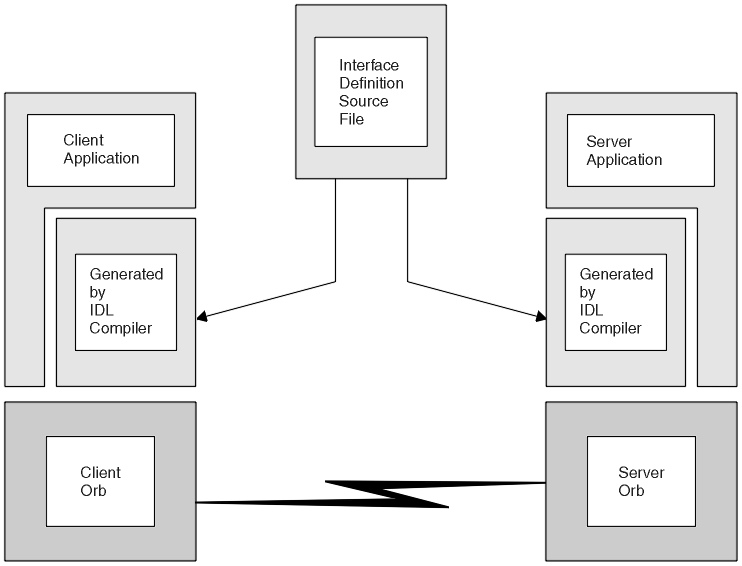
\includegraphics[width=150mm]{img/IDL.png}
\caption{IDL example}
\label{IDL}
\end{figure}

RTI Connext may function as communication layer between the different nodes. Since the \emph{middleware} hides the communication medium from the nodes, the concern of data transportation and distribution is handled by RTI Connext.
Since the RTI Connext is a cross platform and language agnostic, the system will function holisticly across all nodes in the distributed system; and will especially shine in a multi-platform/multi-language environment.

Since RTI Connext is based on DDS, the paradigm is Publish/Subscribe. This paradigm ensures that the nodes only need to know what kind of data they can supply, and what kind of data they need. The whole Publish/Subscribe functionality is handled by RTI Connext. 